\section{The renewal law on the engine}\label{sec:validation}

\begin{figure*}[t]\centering
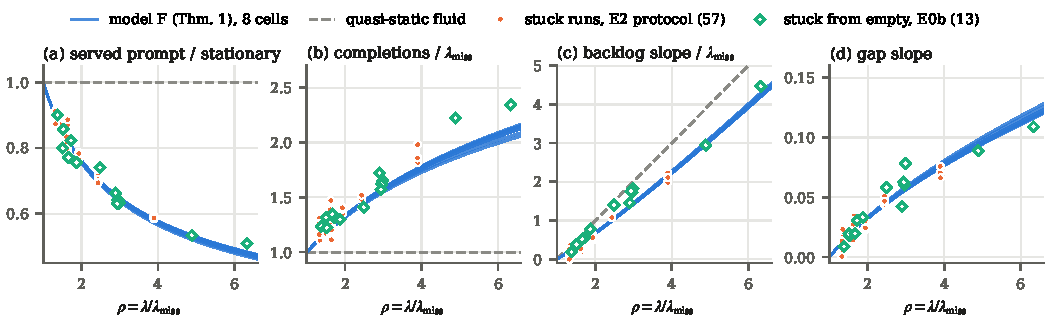
\includegraphics[width=\textwidth]{figs/fig_trap_universality.pdf}
\caption{Theorem~\ref{thm:trap} against every stuck run, as a function of the load $\rho=\lambda/\lmiss$. Points: the 57 stuck
runs of the E2 protocol (orange) and the 13 from-empty runs that were stuck over $[1500,3000)$\,s (E0b, hollow). Lines: model~F
for each of the eight cells; they nearly coincide because the cells' cost-weighted turn mixes are close
($E[T]/\bar k_c=0.60$--$0.62$). No parameter is fitted to any trap measurement. (a)~Mean prompt of the turns served, over the
stationary mean: the tilted turn mix. (b)~Session completion rate over $\lmiss$: the youth premium, above 1. (c)~Backlog growth over
$\lmiss$. (d)~Growth rate of the gap between a session's turns, regressed on the turn's completion time, against model~F's
$\gamma/z=1-1/z$. Dashed: the quasi-static fluid read literally in congestion (stationary composition, completion at $\lmiss$,
growth at $\rho-1$). Retrospective: the theory was derived after these runs were read.}\label{fig:trapuniv}
\end{figure*}

\begin{table*}[t]
\centering\footnotesize
\caption{Evidence ledger: every claim of the paper with its test, its status and the appendix that reports it. Status:
pre-registered or registered as in Table~\ref{tab:stampede}; blind in outcome, predictions frozen before the runs existed (blind
tests use tolerances set on earlier runs); retrospective, theory derived after the runs were read; post hoc, an analysis chosen
after the outcome. Run counts are runs, not independent trials: seeds 0--2 recur across tests. Commits, tags and clock times are
in Appendix~\ref{app:timeline}.}\label{tab:ledger-ev}
\setlength{\tabcolsep}{3pt}
\begin{tabular}{@{}>{\raggedright\arraybackslash}p{4.0cm} >{\raggedright\arraybackslash}p{3.6cm} >{\raggedright\arraybackslash}p{2.9cm} >{\raggedright\arraybackslash}p{5.85cm} c@{}}
\toprule
Claim & Test, runs & Status & Result & App.\\
\midrule
\multicolumn{5}{@{}l}{\emph{The stampede (\S\ref{sec:stampede}); registered and run before Lu et al.'s paper appeared}}\\
A burst traps the engine at a load it carries & E2 in five cells; 30 BURST, 30 NOBURST runs & pre-registered (vLLM registered) & zero hits to the end in 30/30, NOBURST good 30/30; rule met at 9 of 10 rates (Llama 1.35 failed) & \ref{app:stampede}\\
The basin has a size threshold & BASIN-1, BASIN-2; 15 runs & pre-registered & boundary between 40 and 60 sessions in every seed & \ref{app:stampede}\\
A tool slowdown alone can trap & TOOLSLOW; 6 runs & pre-registered & rule not met: +30\,s trapped 1 of 3, +10\,s none & \ref{app:stampede}\\
The trap persists and outlives its trigger & 50 trapped FCFS runs; 16 with the trigger gone & post hoc & no escape in about 100 trapped hours; no hit after the trigger left in 15 of 16 & \ref{app:dataonly}\\
\addlinespace
\multicolumn{5}{@{}l}{\emph{Model~F, retrospective (\S\ref{sec:validation}); nothing fitted to any trap measurement}}\\
The trapped turn mix is $\nu^z$ & 57 E2-protocol stuck runs (30 plans), 13 from empty & retrospective & served prompt within 3\% in 50 of 57 ($-6.6$ to $+7.7$\%) & \ref{app:trapdata}\\
The gap grows linearly, at $1-1/z$ & same & retrospective & pooled median ratio 1.01; per run 0.04--1.81 & \ref{app:trapdata}\\
Completions exceed $\lmiss$ (youth premium) & same & retrospective & every run above $\lref$ (1.10--2.03; 2.40 from empty); 1.08--1.81 net of the token rate & \ref{app:trapdata}\\
The backlog grows at $\alpha$, not $\lambda-\lmiss$ & same & retrospective & slope over $\alpha$: mean 0.99, median 1.06 (quasi-static: 1.36--1.59) & \ref{app:trapdata}\\
\addlinespace
\multicolumn{5}{@{}l}{\emph{Blind tests, registered on 2026-11-05 after Lu et al.'s paper appeared (\S\ref{sec:validation}, \S\ref{sec:control})}}\\
The trap-state law holds on traps with no burst & TOOLSLOW-W (3 stuck), TOOLSLOW-D15 (1 stuck) & pre-registered; blind in outcome & 4 of 5 pre-set scores pass pooled; the per-run slope check failed in 2 of 4 runs & \ref{app:blind}\\
Which seeds a slowdown traps & TOOLSLOW-D15; 3 runs & pre-registered; two frozen predictors & NO-TRAP, as the simulator said per seed; the first-principles fluid verdict (TRAPS) missed & \ref{app:blind}\\
% MIRROR (drop this row if MIRROR is not reported)
A near-deterministic turn count reverses the premium & MIRROR; \pending{runs} & \pending{registration} & \pending{MIRROR outcome} & \ref{app:blind}\\
A cut into $[\lmiss,D)$ does not clear the trap & CUT-A; 3 runs & pre-registered; blind; rule fixed after the predictions were read & pass: theory-favoured 3/3, stuck 3/3; rejects the constant readings only; late slopes post hoc & \ref{app:blind}\\
A cut below $\lmiss$ drains only slowly & CUT-B; 3 runs & as CUT-A & pass: theory-favoured 3/3, backlog falling 3/3, still trapped 3/3 at 8700\,s & \ref{app:blind}\\
\addlinespace
\multicolumn{5}{@{}l}{\emph{The exits (\S\ref{sec:control}); registered before Lu et al.'s paper appeared}}\\
Refusing arrivals drains a trap by shedding & SHED; 4 runs & pre-registered; model~F retrodicted & 600\,s stop stuck 2/2, 3600\,s good 2/2; 355--378 sessions refused & \ref{app:stampede}\\
A cap restores reuse without shedding & R1, R4; 9 runs & pre-registered & rescued 9/9, good after release; 4 of 9 release times outside the frozen $\pm15$\% & \ref{app:stampede}\\
\addlinespace
\multicolumn{5}{@{}l}{\emph{Entry}}\\
The throughput curve from first principles & 8 cells; frozen tags & 5 cells blind (3 in time, 2 by access only, one partly seen) & 0.5-hit crossing off by 1.5 sessions on average (Lu et al.'s curve, read post hoc: 4.1); misses listed & \ref{app:entry}\\
\bottomrule
\end{tabular}
\end{table*}

We test model~F on every trapped run we have, in eight cells: SGLang with the 300k pool (FCFS with and without its waiting-prefix
refresh, the BASIN, SHED and TOOLSLOW runs, and stock LPM past its 128-request fallback), SGLang's native pool, vLLM, the H200 at
300k and 600k, Llama-3.1-8B, and the 150k and 600k pools. Each cell's costs $c_k$ come from the cost model fitted to server-log
iteration timings; vLLM, the H200 and Llama take one speed factor fitted to their own all-miss token rate. No parameter is fitted to
any trap measurement. Table~\ref{tab:ledger-ev} collects the evidence.

\paragraph{Retrospective check.} The theory was derived after these runs had been read, so this check is retrospective, not
blind. Over the 57 stuck runs of the E2 protocol (follow-up hit fraction below 0.2 over $[5700,8700)$\,s; 20 cell and rate groups;
36 runs of registered protocols, on 30 distinct arrival plans; Fig.~\ref{fig:trapuniv}, and per cell Table~\ref{tab:trap} in
Appendix~\ref{app:trapdata}):
\begin{itemize}[leftmargin=*,nosep]
\item \emph{Composition.} The mean prompt of the turns served matches the tilted mix $\nu^z$ to within $-6.6$\% and $+7.7$\%,
and to within 3\% in 50 of the 57 runs. The trapped engine serves turns 10--42\% shorter than the stationary mix, and the
Perron root says by how much.
\item \emph{Gap growth.} The gap between a session's turns grows linearly in time. We regress it on the turn's completion time;
a turn that completes at $t$ joined at about $t/z$, so model~F's slope is $\gamma/z=1-1/z$. Measured over predicted, the ratio has
median 1.01 (mean 0.96). Per run it ranges from 0.04 to 1.81; the low values are the seed-1 runs at 1.35~$\lref$, whose plans
deliver fewer arrivals than nominal (below).
\item \emph{Youth premium.} Every stuck run completes sessions above $\lref$, at 1.10--2.03~$\lref$ (up to 2.40 in the from-empty
runs), and on average 1.055 times $D$ (0.90--1.21). Part of the excess over $D$ is a congested engine computing prompt tokens faster
than the 32-session reference behind $\lref$, most on the H200 and the native pool (Appendix~\ref{app:trapdata}); on vLLM and Llama
the completion excess is not explained. That speed-up does not make the sign: divided by each run's measured token-rate ratio
(0.95--1.12), completions still exceed $\lref$ by a factor of 1.08--1.81 in every one of the 57 runs
(\fpath{analysis/theory/icml/premium_over_tokrate.py}).
\item \emph{Backlog.} Over model~F's $\alpha$, the backlog slope has mean 0.99 and median 1.06 across the 57 runs (per run 0.00
to 1.62, varying mostly with the plans' window arrivals; $\alpha$ at the nominal rate), where the quasi-static equation, completions
at $\lmiss$, gives 1.36--1.59.
\end{itemize}
These are statements about the runs taken together; per run the gap and backlog statistics scatter widely, mostly with the plan's
arrivals over the window. The 13 from-empty runs that were stuck over $[1500,3000)$\,s, at $\rho=1.4$ to 6.3, follow the same
composition and gap laws (composition within $-5.7$\% and $+6.6$\%; gap-slope ratio 0.63--1.37, mean 1.03), but their backlog
slopes run above model~F's $\alpha$, by 6--35\% in 11 of the 13, and their completions by up to 15\%; in model~F the two add up to
the arrival rate, which may reflect window arrival rates above nominal in these single seed-0 runs (3.8--13.1\% above in all 13).
Self-similarity (Theorem~\ref{thm:trap}(b)) is visible only where samples are large and censoring is small
(Appendix~\ref{app:trapdata}).

\paragraph{The registered slope rule, explained post hoc.} Our registered rule calls a BURST run trapped only if its backlog slope
exceeds $0.5(\lambda-\lref)$. At 1.35~$\lref$ Theorem~\ref{thm:trap}(a) puts the true slope at about $0.63(\lambda-\lmiss)$, only
about 25\% above that line, and seed~1's plan delivers 5.8--8.9\% fewer arrivals than nominal over the window at 1.35~$\lref$ in
every cell; 8 of the 9 below-threshold runs are seed~1. The plug-in $\lambda_{\mathrm{window}}(\text{plan})-D$, computable from the
plan before any run, falls on the measured side of the threshold for 27 of the 30 distinct plans of the registered protocols, against
23 for always predicting ``trapped'' (plans of different cells share seeds, so these are not independent trials); two of the three
exceptions lie within $10^{-4}$\,/s of the threshold, and the third is Llama at 1.35~$\lref$, seed~0, the registered failure. This
account is post hoc and changes no registered verdict.

\paragraph{Blind tests of the trap-state law.} The predictions of Theorem~\ref{thm:trap} for runs that did not yet exist were frozen
under tag \texttt{icml-trap-pred} (pushed at 00:24:47 CST on 2026-11-05), with scoring rules S1--S5 declared beforehand: per-run
composition within $\pm8$\% (pooled $\pm5$\%); pooled gap slope within $[0.6,1.4]\gamma$; completion above $\lref$ in every trapped
run at realized load $\ge1.1\lref$ (pooled within $\pm15$\% of $D$); pooled backlog slope within $\pm35$\% of $\alpha$ or of the E2
fluid slope; and, per seed, the plug-in's side of the registered threshold and $|$slope$-$plug-in$|\le0.01$\,/s. The application to a
cell and load is refuted if the pooled S1 or S2 fails in a group of at least two trapped runs
(\fpath{notes/PREDICTIONS_icml_trap.md}). The tolerances were set after seeing the committed runs; the runs they score did not exist
at the push, so these tests are blind in outcome only. Two pre-registered cells trap the engine with no burst; both were designed
after the 900\,s TOOLSLOW arm had trapped 1 of 3 and after reading simulator outputs (Appendix~\ref{app:blind}).
\begin{itemize}[leftmargin=*,nosep]
\item \emph{TOOLSLOW-W}: every tool call that starts in $[1200,3000)$\,s takes 30\,s longer, at 1.35~$\lref$, seeds 0--2, paired
with the committed NOBURST runs; the cell TRAPS if at least 2 of 3 runs are stuck. Outcome: TRAPS. All three runs were stuck (hit
0.000 over $[5700,8700)$\,s; backlog slopes 0.0184--0.0232\,/s against a threshold of 0.0125\,/s) while their paired NOBURST runs stayed
good; on the same plans the 900\,s slowdown had trapped 1 of 3. The pooled scores pass: composition $+1.9$\% (limit $\pm5$\%), gap
slope $1.075\gamma$, completions $+1.9$\% of $D$ with every run above $\lref$, and backlog slope $+29$\% of $\alpha$ (limit
$\pm35$\%). Per run, composition is within $\pm8$\% in all three, and S5's plug-in lies on the measured side of the threshold in 2 of
3 runs and within 0.01\,/s in 3 of 3. Every model we froze predicted this outcome, so the cell tests the trap-state law on a trap
entered with no burst, not the models against each other; it does not separate the longer gap from the capacity loss and the larger
population that come with the slowdown.
\item \emph{TOOLSLOW-D15}: a 15\,s slowdown over $[1200,2100)$\,s at 1.65~$\lref$, chosen so that our two frozen predictors of entry
disagree: the calibrated simulator, run on the exact client plans, called seed~0 stuck and seeds 1 and~2 good (NO-TRAP), while the
first-principles model's plan-averaged fluid verdict called every seed stuck (TRAPS), and its per-seed layer, with the simulator's
modal calls, gave NO-TRAP a probability of 0.41. Outcome: NO-TRAP, as the simulator said, seed by seed: seed~0 stuck, seeds 1 and~2
at their controls' hit rates. The stuck run passed S1--S4 (composition $+0.1$\%, gap slope $1.02\gamma$, completions $+10$\% of
$D$, backlog slope $-15$\% of $\alpha$); its S5 plug-in missed the 0.01\,/s tolerance by 0.0004\,/s, and with one eligible run the
refutation rule does not apply.
\end{itemize}
Across the four blind runs trapped by a tool slowdown alone, S1--S4 pass in both cells, and S5 is close in 3 of 4 and on the correct
side in 3 of 4. The frozen exploratory measures of both cells, hits and misses, are in Appendix~\ref{app:blind}.

% MIRROR: this subsection can be filled from PAPER_INPUT_r16 or dropped whole (also drop the ledger row, the clause in
% contribution (2) and the pointer after Theorem 2).
\subsection{MIRROR: a workload that reverses the premium}\label{sec:mirror}
Theorem~\ref{thm:premium} makes the sign of the premium a property of the workload: for a nearly deterministic turn count the
turn-count factor $H$ is far below 1 and outweighs the cost-growth factor. MIRROR tests this blind. It repeats the E2 BURST protocol
on the 300k A100 cell (1.65~$\lref$ decisive, 1.35~$\lref$ secondary, seeds 0--2, with paired NOBURST runs) with a step-capped
workload, $T=\min(\mathrm{Geometric}(1/1000),20)$, so that about 98\% of sessions run exactly 20 turns; nothing else changes
(\fpath{configs/agentload_e2_mirror_k20.yaml}). For this workload model~F's all-miss capacity is 1.05~$\lref$, and model~F predicts
trapped completions of about $0.77\lmiss$, against a premium of about 23\% for the standard workload; its exact fluid predicts a
near-blackout of completions for about 40\,min after the burst, then a completion wave when the burst cohort finishes its 20th turn,
and a backlog growing about 2.5 times faster than the standard trap. Every throughput-curve reading (the quasi-static model, Lu et
al.'s $\dot N=\lambda-X(N)/K$~\citep{lu2026cachetrap}, our Eq.~\eqref{eq:fluid}) predicts steady completions near the all-miss
capacity instead. The predictions and the decision rule were frozen before the jobs ran \pending{tag, commit and push time; rule in
\fpath{notes/PREDICTIONS_r16_mirror.md}}. Outcome: \pending{MIRROR outcome}.
